\section{The value of a feedback measurement}

A negative definite matrix has a negative Rayleigh quotient in every direction. To rule out negative definiteness, it suffices to find a single direction of positive curvature. This asymmetry suggests a reason to measure adaptively: a weak indication of curvature can guide the next query. How much can such feedback save when each answer is a single noisy real number and even the orientation of the favorable direction is unknown?

\paragraph{Experiment.}
Fix \(m\ge2\), \(0<\gamma\le1/(8\sqrt m)\), and \(0<\delta\le1/8\). The unknown real symmetric matrix \(A\) satisfies \(\|A\|_{\Frob}\le1\) and belongs to one of the two classes
\[
 \Aminus=\{A:\lambda_{\max}(A)\le-\gamma\},\qquad
 \Aplus=\{A:\lambda_{\max}(A)\ge\gamma\}
\]
within this ball. At step \(j\) the test chooses a symmetric \(Q_j\) with \(\|Q_j\|_{\Frob}\le1\) and receives
\begin{equation}\label{eq:observation}
 Y_j=\ip{A}{Q_j}+Z_j,\qquad
 \ip{A}{Q}=\tr(AQ),\qquad Z_j\overset{\mathrm{iid}}{\sim}\N(0,1).
\end{equation}
The noise \(Z_j\) is independent of the preceding observations and of the test's random seed. The unknown matrix stays fixed. A repeated direction therefore costs another observation and reduces the variance of its estimated mean. Computation and storage are unrestricted.

A test stops at \(\tau\) and returns one of the two signs. It is \(\delta\)-correct if its error probability is at most \(\delta\) for each promised input. Write \(\nad\) and \(\nna\) for the infimum of \(\sup_A\E_A\tau\) over such tests with adaptive and nonadaptive designs, respectively. For a nonadaptive design the entire sequence of directions is fixed by the seed, and the decision to stop may depend on the responses. In an \(R\)-batch design, the directions, order, and length of each batch are chosen before its first response. A terminal decision may discard a suffix. Write \(N_R\) for the corresponding minimax cost. All logarithms are natural.

\begin{theorem}[Sample complexity]\label{thm:samples}
Uniformly over the above parameter range, with \(t=\log(1/\delta)\),
\begin{align}
 \nad(m,\gamma,\delta)&=\Theta\!\left(\frac{m^2}{\gamma^2}(\log m+t)\right),\label{eq:ad}\\
 \nna(m,\gamma,\delta)&=\Theta\!\left(\frac{m^2}{\gamma^2}(m+t)\right).\label{eq:na}
\end{align}
The upper bounds hold with deterministic observation budgets. The constants in both bounds are universal.
\end{theorem}

For fixed risk, the ratio \(\nna/\nad\) is of order \(m/\log m\). For \(\log m\le t\le m\) it is of order \(m/t\). Once \(t\ge m\), the cost of certifying the sign already pays for a one-batch reconstruction in operator norm. \Cref{fig:regimes} plots the ratio of the two rate expressions across these regimes.

\begin{figure}[htbp]
 \centering
 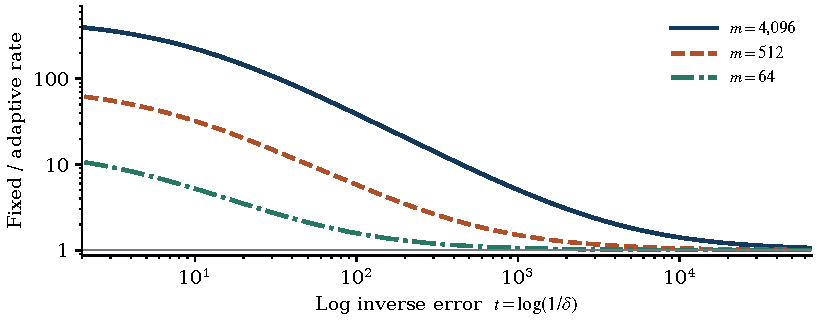
\includegraphics[width=.85\linewidth]{figures/confidence.pdf}
 \caption{Feedback gain as a function of the required confidence. Each curve shows \((m+t)/(\log m+t)\), the ratio in \cref{thm:samples} up to universal constants. The horizontal coordinate is \(t=\log(1/\delta)\). Both axes are logarithmic.}\label{fig:regimes}
\end{figure}

The worst-case rate hides a difference between the two answers. Let \(N_+\) and \(N_-\) be the respective infima of \(\sup_{A\in\Aplus}\E_A\tau\) and \(\sup_{A\in\Aminus}\E_A\tau\) over adaptive tests that meet the error requirement on both classes and have finite worst-case expected cost.

\begin{theorem}[Cost on each sign]\label{thm:classwise}
One test simultaneously attains the two minimax expected costs, up to universal constants,
\[
 N_+=\Theta\!\left(\frac{m^2\log m+t}{\gamma^2}\right),\qquad
 N_-=\Theta\!\left(\frac{m^2(\log m+t)}{\gamma^2}\right).
\]
On every run its cost is at most \(C m^2(\log m+t)/\gamma^2\).
\end{theorem}

Both signs require an initial search. On a positive input, the algorithm can extract a unit vector \(v\) with \(v^\top A v\ge\gamma/48\) at constant success probability. Fresh measurements along \(vv^\top\) can then validate that direction. The proof in \cref{sec:classwise} turns this observation into a single stopping rule for both signs.

\begin{theorem}[Number of feedback batches]\label{thm:rounds}
There are universal constants \(c,C>0\) such that for every \(R\ge1\),
\[
 N_R(m,\gamma,1/8)\ \ge\ c\,e^{-CR}\frac{m^3}{\gamma^2}.
\]
In particular every fixed number of batches has cost \(\Theta_R(m^3/\gamma^2)\). For fixed \(\varepsilon>0\), any family of tests with cost \(O(m^{3-\varepsilon}/\gamma^2)\) needs \(\Omega_\varepsilon(\log m)\) batches.
\end{theorem}

The sample-optimal adaptive test below uses \(O(\log m\max\{1,(m/(\log m+t))^{1/4}\})\) batches. For \(t\ge m\), the one-batch design already attains the optimal worst-case sample rate. Determining the least number of batches that attains \eqref{eq:ad} on the full matrix class remains open in the fixed-risk regime.

\paragraph{How the sign enters the lower bound.}
The difficult instances share a Gaussian matrix drawn once at the start of the experiment. On the positive side a rank-one perturbation competes with this background. Repeating a query averages away its observation noise while preserving the contribution of the background. For a fixed design one can whiten the entire response vector. With feedback the design itself depends on the unknown perturbation. We control how fast the transcript acquires information about its two factors, then translate that control into a bound on the distance between the positive and negative transcript laws. This last step matters because a test can in principle identify the sign while learning little about either factor.

\paragraph{Connections to earlier work.}
The change of variables \(M=-A-\gamma I\) maps the negative class to a positive semidefinite matrix and the positive class to \(\lambda_{\min}(M)\le-2\gamma\). Needell, Swartworth and Woodruff~\cite{needell2022} established adaptive and nonadaptive separations for positive semidefiniteness testing with exact queries. Their Theorem~31 and Remark~32 use the shifted dilation of a spiked Gaussian matrix and draw on the sketching lower bound of Li and Woodruff~\cite{li2016}. We use that family here. With fresh noise and repeated queries, the squared eigenvalues of a contracted design Gram matrix determine the fixed-design mixture bound. Nenadov and Verlinde~\cite{nenadov2026} study a complementary access model in which a random principal submatrix reveals a violation when the input is sufficiently far from the positive semidefinite cone in normalized Frobenius distance.

Feedback also changes the complexity of recovering a principal subspace from exact matrix--vector products~\cite{simchowitz2018}, recovering low-rank matrices under orthonormal sensing designs~\cite{kacham2024}, and identifying a nearly optimal arm in a linear bandit~\cite{maiti2026}. Here a matrix--vector product already costs \(m\) scalar measurements. The output is one bit, and the alternative allows a full-rank matrix with an unknown leading eigenspace. A lower bound for recovering that eigenspace would require an additional reduction to apply to this decision problem.

General-answer linear pure exploration gives an earlier explanation for the high-confidence asymmetry. For fixed \(m,\gamma\), the characteristic time of Degenne et al.~\cite{degenne2020} on a spanning design containing a fine net of rank-one directions has worst-case order \(\gamma^{-2}\) on positive inputs and \(m^2\gamma^{-2}\) on negative inputs. A near-maximizing direction separates a positive input from every negative one. On a negative input, uniform basis measurements suffice, and the spherical average in \eqref{eq:sph} gives the matching obstruction. Their asymptotic result holds as \(\delta\) tends to zero with the design fixed. \Cref{thm:classwise} identifies the discovery cost and gives rates uniform in all three parameters.

On the algorithmic side, the second-moment estimate of Gu et al.~\cite{gu2026} already leads to an \(O(m^2\log^2m/\gamma^2)\) fixed-risk test in this model. We give the reduction in \cref{sec:oja}. Our construction rescales the spectrum using a coarse estimate, in the spirit of absolute-value preconditioning~\cite{vecharynski2013}, and implements a block Chebyshev recurrence with noisy scalar probes. Under the null a quadratic energy controls its upper tail. Under the alternative an inverse moment of the growing component controls its lower tail. These two estimates give the additive \(\log m+\log(1/\delta)\) dependence in \eqref{eq:ad}.
